\documentclass[12pt]{article}

\usepackage[margin=1in,includefoot]{geometry}
\pagenumbering{gobble}
\usepackage{textcomp}
\usepackage[utf8]{inputenc}
\usepackage{amsmath}
\usepackage{amssymb}
\usepackage{mathabx}
\usepackage{enumitem}
\usepackage[utf8]{inputenc}
\usepackage{listings}
\usepackage{graphicx}
\graphicspath{ {/Users/Mac/Desktop} }
\usepackage{tikz}
\usepackage{pgfplots}

\begin{document}

\title{COMP1100 Assignment 1 Report}
\author{Name and ID: Alexander Jones U5956709 \hfil Tutor: Nathan Yong}
\date{22 April 2016}
\maketitle

\tableofcontents

\section{Rationale for Program Design}

I decided to keep things simple and readable. Throughout my program I use helper functions and split each task into the smallest possible components to keep my program clearn, readable and easy to modify.

I faced many challenges on the way to producing a working program. I had some trouble getting part 1 to work properly because I did not complete understand how to modify record types and especially nexted records (i.e., SquareWorld is a nested record of Ant, which itself is a nested record of Coord). I went back to basics and re-learnt how to modify records. The way I dealt with the nesting is by making helper functions that modify the antPosition and antOrientation at the smallest scale possible and then combining these helper function up to procuce a new SquareWorld with the required modifications.

It is possible to do turnAnt and moveAnt without helper functions but I find that to be extremely unreadable and difficult to understand. It also makes it difficult to modify or fix. Having helper functions make the code more modular as I can just copy past my part 0 functions to part 2 and make simple modifications.

The biggest challenge was getting part 1 to produce the correct output. For about 5 days, I struggled to get art one to procuce the correct output. Here are the wrong outputs that I was getting:

\break

\begin{itemize}
\item the ant would go around in a circle changing only the square it is on
\item the ant would create a diagonal of blue squares that goes forever
\item the ant would 4 blue squares in the middle of the screen and not make any new squares
\end{itemize}

My proram was able to get the correct turns because the ant turned L on blue squares and R on red squares so there was no problem with my genSquareTurn function. My program was moving the ant forward and changing its direction so there was no problem with moveAnt and turnAnt (as confirmed by part 0) so the problem must have been with updating the world.

Initially, when I added new cells to the world, I did not remove the old cell because I thought that was done automatically so I used list comprehension to remove the old cell and add a modified cell but this alone did not solve the problem. My original genCurrentCell was wrong because I had the following case in it:

\begin{lstlisting}
[] -> [Cell {cellPosition = Coord {xCoord = 0, yCoord = 0},
cellState = defaultState}]
\end{lstlisting}

The problem with this was that whenever the ant has not visited a cell previously, this above cell is returned which is just the cell at coord (0,0) with colour black, which is wrong. I then updated my genCurrentCell function to be called only if I definitely know that the cell I am looking for exists in theWorld. I determine existence of cell by using a combination of

\begin{lstlisting}
checkCellExistence :: SquareWorld -> Bool
\end{lstlisting}

located in src/StudentSources/LangtonsAnt.hs and the provided function findCell.

\hfill

Another challenge I faced was getting the correct SquareTurn value without having to hard code it. If I hard coded it then the program would only work for Langton's Ant but I wanted it to work for other transition systems.

I looked through the Main.hs file and found a very helpful like:

\begin{lstlisting}
let trans = case getArg args Trans of
  Nothing -> [R,L]
\end{lstlisting}

This made me realise that all the transition rules are stored in the antTransition in the [Transition SquareTurn] list. So I made a function called genSquareTurn which compared the colour of the current cell with the colours in the transitions list using pattern matching and procuces the correct SquareTurn using the turnDirection accessor function.

This meant that my program can work for any transition system that we can input using readSquareTransition.

\break

I then went back to basics and listed the steps I need to take to get my program to produce the correct output:

\begin{enumerate}
\item check if the ant visited the cell previously (i.e. a cell with cellPosition = antPosition exists in theWorld). This can be done using the provided function findCell located in src/Datastructures/SquareWorld.hs and a helper function called checkCellExistence.
\item If the ant visited a cell previously, then remove it from the world and replace it with a new cell that has the same position as the ant and cellState = nextCellState currentState.
\item If the ant has not visited the cell previously, then create a new cell with the same position as the ant and cellState = nextCellState defaultState. This is because if the ant never visited that cell previously, then it must be black (i.e. it has cellState = defaultState) so we change it into the following state using nextCellState. There is no need to remove any cells in this case because there is no change of having duplicate cells in the world.
\item The able two cases will both produce SquareWorld values with theWorld field updates to either replace a cell or add a new cell.
\item This new SquareWorld value along with a SquareTurn value generated using the genSquareTurn function are passed into turnAnt function from part 0 to produce a SquareWorld value with the ant turned.
\item This new SquareWorld value is then passed to moveAnt to procude the final SquareWorld value that is then outputed by the transitionWorld function.
\end{enumerate}

Using the above steps I was able to produce a working program. I tested the program with different transition systems other than Langton's ant ant it works as expected.

I compared my performace with other classmates and my program produces comparable time results so I believe that my choice to make the program as readable as possible did not compromise performance in any major way.

My program has limitations and areas which I could improve.
For example, I hard coded all possible combinations of HexTurn and HexDirection for the updateAntDirection function in src/SturentSources/LangtonsHex. This does not look very elegant. i tried to find an alternative way to generalise the function and do it more elegantly but couldn't.

Completing part 2 was very simple once I completed part 1.
The only challenge i faced while completing part 2 was writing the readHexTransition function because of the variable length of HexTurn values. Then I realised it can be done the same way as readSquareTransition using pattern matching. For both readSquareTransition and readHexTransition I had to make a function called unMaybefyList which removed the Maybe type from a list. This was done to be able to recurse through the input string and add new HexTurn values to the output list.

\break

\section{Program Performance}

\hfil

\noindent \large{\textbf{Afew time measurements for Langton's Square: }}

\begin{lstlisting}
$./run_langtons_ant -m square
After 5000 transitions the ant is at
Coord {xCoord = 2, yCoord = -10}
and it took us 0.12636s to calculate that
$ ./run_langtons_ant -m square --time 10000
After 10000 transitions the ant is at
Coord {xCoord = -16, yCoord = 10}
and it took us 0.416684s to calculate that
$ ./run_langtons_ant -m square --time 25000
After 25000 transitions the ant is at
Coord {xCoord = -306, yCoord = -282}
and it took us 2.542863s to calculate that
$ ./run_langtons_ant -m square --time 50000
After 50000 transitions the ant is at
Coord {xCoord = -784, yCoord = -764}
and it took us 11.232911s to calculate that
$./run_langtons_ant -m square --time 75000
After 75000 transitions the ant is at
Coord {xCoord = -1266, yCoord = -1240}
and it took us 26.818762s to calculate that
$./run_langtons_ant -m square --time 100000
After 100000 transitions the ant is at
Coord {xCoord = -1748, yCoord = -1726}
and it took us 50.495255s to calculate that
\end{lstlisting}

\break

\noindent \large{\textbf{Afew time measurements for Langton's Hex: }}

\begin{lstlisting}
$ ./run_langtons_ant -m hex
After 5000 transitions the ant is at
Coord {xCoord = -17, yCoord = 7}
and it took us 0.105311s to calculate that
$ ./run_langtons_ant -m hex --time 10000
After 10000 transitions the ant is at
Coord {xCoord = -10, yCoord = -10}
and it took us 0.325092s to calculate that
$ ./run_langtons_ant -m hex --time 25000
After 25000 transitions the ant is at
Coord {xCoord = -1, yCoord = -1}
and it took us 1.546423s to calculate that
$ ./run_langtons_ant -m hex --time 50000
After 50000 transitions the ant is at
Coord {xCoord = -8, yCoord = 4}
and it took us 5.019095s to calculate that
$./run_langtons_ant -m hex --time 75000
After 75000 transitions the ant is at
Coord {xCoord = 5, yCoord = 8}
and it took us 10.554683s to calculate that
$./run_langtons_ant -m hex --time 100000
After 100000 transitions the ant is at
Coord {xCoord = -3, yCoord = -3}
and it took us 18.637697s to calculate that
\end{lstlisting}

\break

\large{\textbf{Plot for Langton's Hex: }}

\hfil

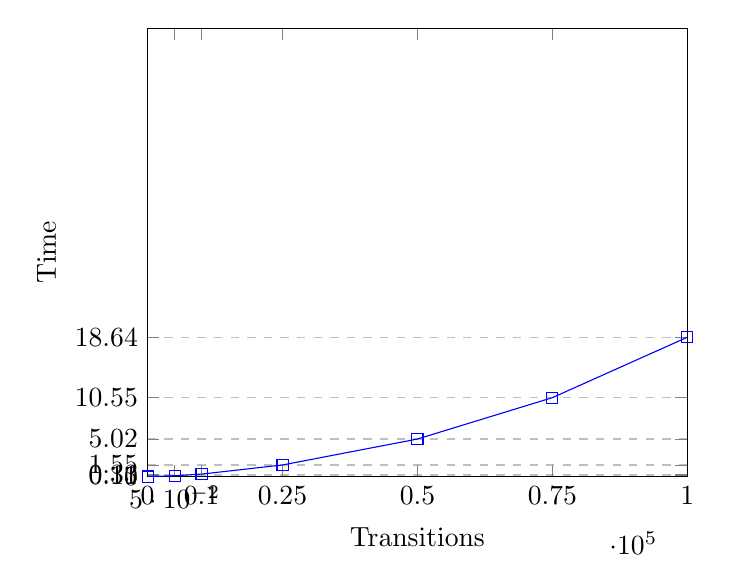
\begin{tikzpicture}
\begin{axis}[
    xlabel={Transitions},
    ylabel={Time},
    xmin=0, xmax=100000,
    ymin=0, ymax=60,
    xtick={0,5000,10000,25000,50000,75000,100000},
    ytick={0,0.1053,0.3251,1.5464,5.0191,10.5547,18.6377},
    legend pos=north west,
    ymajorgrids=true,
    grid style=dashed,
]
 
\addplot[
    color=blue,
    mark=square,
    ]
    coordinates {
    (0,0)(5000,0.1053)(10000,0.3251)(25000,1.5464)(50000,5.0191)(75000,10.5547)(100000,18.6377)
    };
 
\end{axis}
\end{tikzpicture}

\large{\textbf{Plot for Langton's Square: }}

\hfil

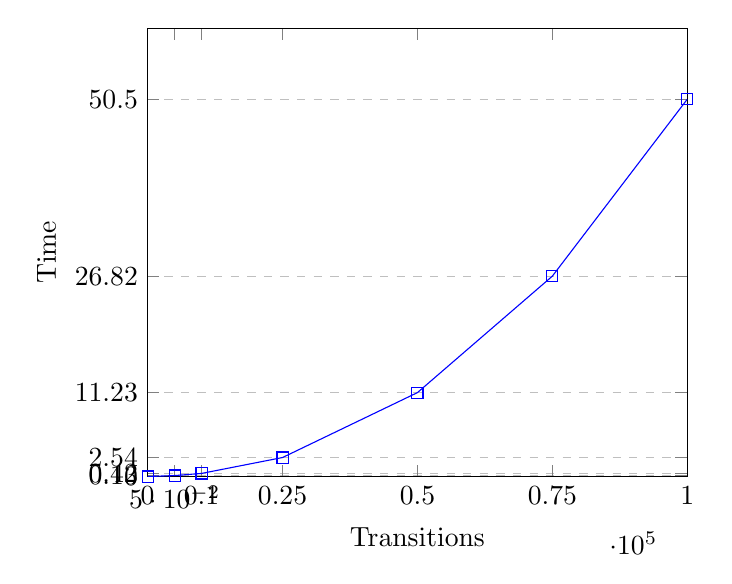
\begin{tikzpicture}
\begin{axis}[
    xlabel={Transitions},
    ylabel={Time},
    xmin=0, xmax=100000,
    ymin=0, ymax=60,
    xtick={0,5000,10000,25000,50000,75000,100000},
    ytick={0,0.1264,0.4167,2.5429,11.2329,26.8188,50.4953},
    legend pos=north west,
    ymajorgrids=true,
    grid style=dashed,
]
 
\addplot[
    color=blue,
    mark=square,
    ]
    coordinates {
    (0,0)(5000,0.1264)(10000,0.4167)(25000,2.5429)(50000,11.2329)(75000,26.8188)(100000,50.4953)
    };
 
\end{axis}
\end{tikzpicture}

\break

\large{\textbf{Analysis of Measurements: }}

As we can see from the graphs, time taken to calulate transitions increases exponentially for both Square and Hex but at a slower rate for Hex. This is expected because as the world gets larger, the list of cells also gets larger and searching the list of cells to find the current cells to modify it or to add new cells would take increasingly more time because I am not using any cleaver searching algorithms, i am just going through the list until the cell is found.  If the cell is not found, then I have to go through the entire list until I reach the empty list.

For Langton's Square, the measurements match my expectations because most other students I tanked to got comparable results, some a bit faster. However, I expected Langton's Hex to take longer than Langton's Square because there are more turns to consider and more ways to modify the coordinate.

There are many things I would do to speed up my program. Fir of all, i would use a faster searching algorithm to find the current cell in theWorld or if the cell does not yet exist in theWorld. To do this, I would use a sorted list of cell, sorted by cellPosition and then use an algorithm like binary search which uses divide and conqure to reduce the time taken to find the cell by not having to search the hald of the list that definitely does not contain the coordinate we want.

Another thing I can do to increase the performance of my program is to get rid off all cells with colour zero and not include them in the list of cells because the background of the grid is black so a black cell doesn't need to be stored. If the ant visits a black cell, then the False case is activated in transitionWorld and the black cell is turned on.

If I had the time, I would use a completely different data structure to make my program faster like a self balancing binary tree. The reason for this is that at every node in the tree we can choose to go left or right depending on the item we are searching for, which reudces time complexity compared to a list. Look ups in a self balancing binary tree are O(logN) compared with O(N) for lists. Another data structure that can be used is a hash table but I am not sure if it is suitable for this program in particular. Look ups for hash tables are O(1).

\break

\section{Extension}

Not Applicable for COMP1100

\break

\section{What Did You Learn?}

\hfill

I learnt many useful things during the course of completing this assignment. It was one of the best assignments I have done so far and I am planning on doing some of the extensions later just out of interest and curiosity.

The part that I spent the most time with was part 1. Part 1 was the biggest hurdle in this assignment for me and the most enjoyment I had during this assignment was when my program finally produced an ant that followed Langton's rules properly. Once I got my part 1 working, it took me about 1 hour to complete part 2.

Being able to simply copy and paste functions from part 1 to part 1 showed me the power of modularity of functional programming.

After this I spent a lot of time trying different transition systems that produced very interesting results such as:

\begin{enumerate}
\item RLR, LLR, LRRRRRLLR, LLRRRLRLRLLR and RRLLLRLLLRRR for Square
\item L2NNL1L2L1, L1L2NUL2L1R2 and R1R2NUR2R1L2 for Hex
\end{enumerate}

Reference: en.wikipedia.org/wiki/Langton%27s_ant

The greatest thing about this assignment was the satisfaction of producing a working program that actually does something interesting.

I feel much more comfortable in my ability to write functions in Haskell after I completed this assignment. I now have a solid understanding of pattern matching, how to divide a problem down into smaller parts using helper functions and I also have a solid understanding of how Maybe types, lists and strings work in haskell. I found working with functions and recursion to be very powerful and enjoyable. I believe that my Haskell programming skills improved the most during the course of this assignment.

Another important skill that I learnt is to appreciate the importace of writing clean and readable code. I used many helpter functions and where syntax.

I decided to do my report completely in LaTeX, which was a very useful experience because I learnt many useful LaTeX techniques in the process such as generating plots from data, inseting source code and so on.

\end{document}